% !TeX program = lualatex
% !TeX encoding = UTF-8
\documentclass[10pt, aspectratio=169, t]{beamer}
\usepackage{fontspec}
\usepackage{polyglossia}
\usepackage[european]{circuitikz}
\usepackage{booktabs}

% Налаштування мов
\setmainlanguage{polish}
\setotherlanguage{english}

% Основні пакети
\usepackage{microtype}
\usepackage{graphicx}
\usepackage{amsmath, amssymb}
\usepackage{xcolor}
\usepackage{tikz}

% Użycie motywu Berlin
\usetheme{Berlin}

% Nagłówek i stopka
\setbeamertemplate{navigation symbols}{}
\setbeamertemplate{footline}[page number]

\title{Modelowanie nagrzewania silnika elektrycznego z wykorzystaniem równań różniczkowych}

\author{Omeliukh Vitalii (181517) \and Dmytro Pavlyk (181518)}
\institute{Kierunek: Inżynieria i Analiza Danych}
\date{\today}

\begin{document}
	
	
	
	% Slajd tytułowy
	\begin{frame}
		\titlepage
		
		\vspace{0.5cm}
		\begin{center}
			
\includegraphics[height=2.5cm]{wmifs_pl.png}
		\end{center}
		\vspace{0.5cm}
	\end{frame}
	
	
	% План презентації
% Plan prezentacji
\begin{frame}
	\frametitle{Plan prezentacji}
	
	\begin{enumerate}
		\item Cel projektu i motywacja
		\item Opis zjawiska nagrzewania silnika
		\item Model matematyczny (bilans cieplny)
		\item Równanie różniczkowe układu
		\item Rozwiązanie analityczne
		\item Implementacja w programie Maxima
		\item Wyniki symulacji – wykresy
		\item Podsumowanie i wnioski
	\end{enumerate}
\end{frame}



% Slajd: Cel projektu
\begin{frame}
	\frametitle{Cel projektu}
	
	\begin{center}
		\textbf{Modelowanie termiczne silnika elektrycznego} \\
		za pomocą równania różniczkowego
	\end{center}
	
	\vspace{0.3cm}
	
	\begin{columns}[T]
		\begin{column}{0.5\textwidth}
			\begin{block}{Cele analityczne}
				\begin{itemize}
					\item Wyprowadzenie równania z bilansu energii
					\item Rozwiązanie analityczne
					\item Interpretacja fizyczna
				\end{itemize}
			\end{block}
			
			\begin{block}{Cele symulacyjne}
				\begin{itemize}
					\item Implementacja w Maxima
					\item Generacja wykresów
					\item Analiza parametrów
				\end{itemize}
			\end{block}
			
			\begin{exampleblock}{Pytanie badawcze}
				\textbf{Jak zmiana obciążenia silnika (parametru $P$)} wpływa na:
				\begin{itemize}
					\item temperaturę pracy?
					\item bezpieczeństwo eksploatacji?
				\end{itemize}
			\end{exampleblock}
		\end{column}
		
		\begin{column}{0.5\textwidth}
			\begin{block}{Parametry modelu}
				\[
				\begin{aligned}
					P &- \text{moc strat [W]} \\
					R_{th} &- \text{rezystancja termiczna [K/W]} \\
					C_{th} &- \text{pojemność cieplna [J/K]} \\
					T_a &- \text{temperatura otoczenia [°C]}
				\end{aligned}
				\]
			\end{block}
			\vspace{-0.3cm}
			\begin{alertblock}{Badany parametr}
				\centering
				\vspace{0.1cm}
				\textbf{$P$ – moc strat cieplnych silnika [W]} \\
				\small(związana z jego obciążeniem)
				\vspace{0.1cm}
			\end{alertblock}
			
			\begin{block}{Zastosowanie praktyczne}
				\begin{itemize}
					\item Projektowanie silników
					\item Dobór układów chłodzenia
					\item Bezpieczna eksploatacja
				\end{itemize}
			\end{block}
		\end{column}
	\end{columns}
\end{frame}



% Slajd: Model matematyczny – założenia
\begin{frame}
	\frametitle{Model matematyczny – założenia}
	
	\begin{columns}[T]
		\begin{column}{0.55\textwidth}
			\begin{block}{Założenia uproszczające}
				\begin{itemize}
					\item Jednorodna temperatura silnika $T(t)$
					\item Stała moc strat cieplnych $P$
					\item Stała temperatura otoczenia $T_a$
					\item Liniowa wymiana ciepła
					\item Stałe parametry $R_{th}$, $C_{th}$
				\end{itemize}
			\end{block}
			\vspace{-0.3cm}
			\begin{block}{Analogia elektryczna}
				Model termiczny $\leftrightarrow$ Obwód RC
				\begin{itemize}
					\item $P$ $\leftrightarrow$ źródło prądu
					\item $R_{th}$ $\leftrightarrow$ rezystor
					\item $C_{th}$ $\leftrightarrow$ kondensator
					\item $T$ $\leftrightarrow$ napięcie
				\end{itemize}
			\end{block}
		\end{column}
		
		\begin{column}{0.45\textwidth}
			\begin{center}
				\begin{tikzpicture}[scale=0.9]
					% Obwód analogii elektrycznej
					\draw[thick] (0,0) to[I, l=$P$, *-*] (0,2);
					\draw[thick] (0,2) -- (2,2);
					\draw[thick] (2,2) to[R, l=$R_{th}$, *-*] (2,0);
					\draw[thick] (2,2) -- (4,2);
					\draw[thick] (4,2) to[C, l=$C_{th}$, *-*] (4,0);
					\draw[thick] (4,0) -- (0,0);
					
					% Temperatura
					\node at (3,1) {$T(t)$};
					\draw[<->, blue, thick] (2.2,1.8) -- (3.8,1.8);
					
					% Ziemia
					\draw (0,0) node[ground]{};
					\node[left] at (0,0) {$T_a$};
				\end{tikzpicture}
				
				\vspace{0.3cm}
				\textbf{Analogia obwodu RC}
			\end{center}
		\end{column}
	\end{columns}
\end{frame}



% Slajd: Bilans energii termicznej
\begin{frame}
	\frametitle{Bilans energii termicznej}
	
	\begin{block}{Podstawowe równanie bilansu}
		\[
		\boxed{C_{th}\frac{dT}{dt} = P - \frac{T - T_a}{R_{th}}}
		\]
	\end{block}
	
	\vspace{-0.3cm}
	
	\begin{columns}[T]
		\begin{column}{0.45\textwidth}
			\begin{block}{Parametry modelu}
				\centering
				\tiny
				\setlength{\tabcolsep}{1pt}
				\begin{tabular}{@{}p{0.9cm}p{1.8cm}@{}}
					\hline
					\textbf{Symb.} & \textbf{Opis} \\
					\hline
					$T(t)$ & Silnik [°C] \\
					$T_a$ & Otoczenie [°C] \\
					$P$ & Moc strat [W] \\
					$R_{th}$ & R term. [K/W] \\
					$C_{th}$ & Pojemność [J/K] \\
					\hline
				\end{tabular}
			\end{block}
			
			\begin{exampleblock}{Składniki}
				\tiny
				\begin{itemize}
					\item $C_{th}\dfrac{dT}{dt}$ – zmiana energii
					\item $P$ – nagrzewanie
					\item $\dfrac{T-T_a}{R_{th}}$ – chłodzenie
				\end{itemize}
			\end{exampleblock}
		\end{column}
		
		\begin{column}{0.55\textwidth}
			\begin{alertblock}{Interpretacja fizyczna}
				\tiny
				\begin{itemize}
					\item $P$ duże → szybkie nagrzewanie
					\item $R_{th}$ duże → słabe chłodzenie
					\item Stan równowagi: $T = T_a + PR_{th}$
					\item Czas nagrzewania: $\tau = R_{th}C_{th}$
				\end{itemize}
			\end{alertblock}
			
			\vspace{0.1cm}
			
			\begin{block}{Sens równania}
				\tiny
				Bilans między:
				\begin{itemize}
					\item Ciepłem wytwarzanym ($P$)
					\item Ciepłem oddawanym
					\item Zmianą temperatury
				\end{itemize}
			\end{block}
		\end{column}
	\end{columns}
	
	\vspace{0.1cm}
	
	\begin{center}
		\scriptsize
		\textbf{Temperatura ustalona:} $T_\infty = T_a + PR_{th}$ \quad \textbf{Stała czasowa:} $\tau = R_{th}C_{th}$
	\end{center}
\end{frame}
%
%
%
%% Slajd: Rozwiązanie analityczne (wersja skrócona)
%\begin{frame}
%	\frametitle{Rozwiązanie analityczne równania}
%	
%	Równanie różniczkowe:
%	\[
%	\frac{d\theta}{dt} + \frac{1}{\tau}\theta = \frac{P}{C_{th}}, 
%	\qquad \tau = R_{th}C_{th}
%	\]
%	
%	Rozwiązanie:
%	\[
%	\theta(t) = P R_{th} + (\theta_0 - P R_{th}) e^{-t/\tau}
%	\]
%	
%	Zależność między temperaturą a przyrostem:
%	\[
%	T(t) = T_a + \theta(t)
%	\]
%	
%	Ostatecznie:
%	\[
%	T(t) = T_a + P R_{th} + (T_0 - T_a - P R_{th}) e^{-t/\tau}
%	\]
%\end{frame}
%
%
%
%% Slajd: Wnioski z rozwiązania
%\begin{frame}
%	\frametitle{Wnioski z rozwiązania}
%	
%	Temperatura ustalona silnika:
%	\[
%	T_\infty = T_a + P R_{th}
%	\]
%	
%	Stała czasowa nagrzewania:
%	\[
%	\tau = R_{th} C_{th}
%	\]
%	
%	\begin{itemize}
%		\item Większa moc strat $P$ powoduje wzrost temperatury pracy silnika.
%		\item Większe $R_{th}$ lub $C_{th}$ oznaczają wolniejsze nagrzewanie.
%		\item Parametry $R_{th}$ i $C_{th}$ decydują o dynamice procesu cieplnego.
%	\end{itemize}
%\end{frame}





%% Slajd: Bilans energii termicznej
%\begin{frame}
%	\frametitle{Bilans energii termicznej}
%	
%	\begin{block}{Równanie bilansu cieplnego}
%		\[
%		\boxed{
%			C_{th}\frac{dT(t)}{dt}
%			=
%			P - \frac{T(t) - T_a}{R_{th}}
%		}
%		\]
%	\end{block}
%	
%	\vspace{-0.2cm}
%	
%	\begin{columns}[T]
%		\begin{column}{0.45\textwidth}
%			\begin{block}{Znaczenie składników}
%				\small
%				\begin{itemize}
%					\item $C_{th}\dfrac{dT}{dt}$ – akumulacja energii cieplnej
%					\item $P$ – moc strat (źródło ciepła)
%					\item $\dfrac{T - T_a}{R_{th}}$ – oddawanie ciepła do otoczenia
%				\end{itemize}
%			\end{block}
%		\end{column}
%		
%		\begin{column}{0.55\textwidth}
%			\begin{alertblock}{Interpretacja fizyczna}
%				\small
%				\begin{itemize}
%					\item im większe $P$ – tym szybsze nagrzewanie
%					\item większe $R_{th}$ – słabsze chłodzenie
%					\item równowaga: $\displaystyle T = T_a + P R_{th}$
%					\item stała czasowa: $\displaystyle \tau = R_{th} C_{th}$
%				\end{itemize}
%			\end{alertblock}
%		\end{column}
%	\end{columns}
%	
%\end{frame}

% Slajd: Uproszczenie zapisu równania
\begin{frame}
	\frametitle{Postać równania różniczkowego}
	
	\begin{block}{Przyrost temperatury}
		W celu uproszczenia zapisu wprowadzamy przyrost temperatury
		względem otoczenia:
		\[
		\theta(t) = T(t) - T_a
		\]
	\end{block}
	
	\vspace{0.2cm}
	
	\begin{block}{Równanie różniczkowe układu}
		\[
		\frac{d\theta(t)}{dt}
		+
		\frac{1}{R_{th} C_{th}} \, \theta(t)
		=
		\frac{P}{C_{th}}
		\]
	\end{block}
	
	\vspace{0.1cm}
	
	\begin{center}
		\small
		\[
		\tau = R_{th} C_{th}
		\quad \Rightarrow \quad
		\frac{d\theta}{dt} + \frac{1}{\tau}\theta = \frac{P}{C_{th}}
		\]
	\end{center}
	
\end{frame}

% Slajd: Rozwiązanie analityczne
\begin{frame}
	\frametitle{Rozwiązanie analityczne}
	
	\begin{block}{Rozwiązanie równania}
		Rozwiązaniem liniowego równania różniczkowego jest:
		\[
		\theta(t)
		=
		P R_{th}
		+
		\bigl(\theta_0 - P R_{th}\bigr)
		e^{-t/\tau}
		\]
	\end{block}
	
	\vspace{0.2cm}
	
	\begin{block}{Powrót do temperatury silnika}
		\[
		T(t) = T_a + \theta(t)
		\]
	\end{block}
	
	\vspace{0.1cm}
	
	\begin{center}
		\small
		\[
		\boxed{
			T(t)
			=
			T_a + P R_{th}
			+
			\bigl(T_0 - T_a - P R_{th}\bigr)
			e^{-t/\tau}
		}
		\]
	\end{center}
	
\end{frame}






\begin{frame}
	\frametitle{Wykres: Temperatura silnika}
	
	\begin{columns}[T]
		% --- Lewa kolumna: parametry ---
		\begin{column}{0.38\textwidth}
			\textbf{Parametry:}
			\vspace{0.2cm}
			\begin{itemize}
				\item $T_a = 20^\circ$C
				\item $T_0 = 20^\circ$C
				\item $R_{th} = 2\ \text{K/W}$
				\item $C_{th} = 5\ \text{J/K}$
				\item $P \in \{50,\ 150\}\ \text{W}$
			\end{itemize}
			
			\vspace{0.2cm}
			{\footnotesize
				Wykres przedstawia przebieg temperatury $T(t)$ w czasie dla dwóch wartości mocy strat $P$.
			}
		\end{column}
		
		% --- Prawa kolumna: obrazek ---
		\begin{column}{0.62\textwidth}
			\centering
			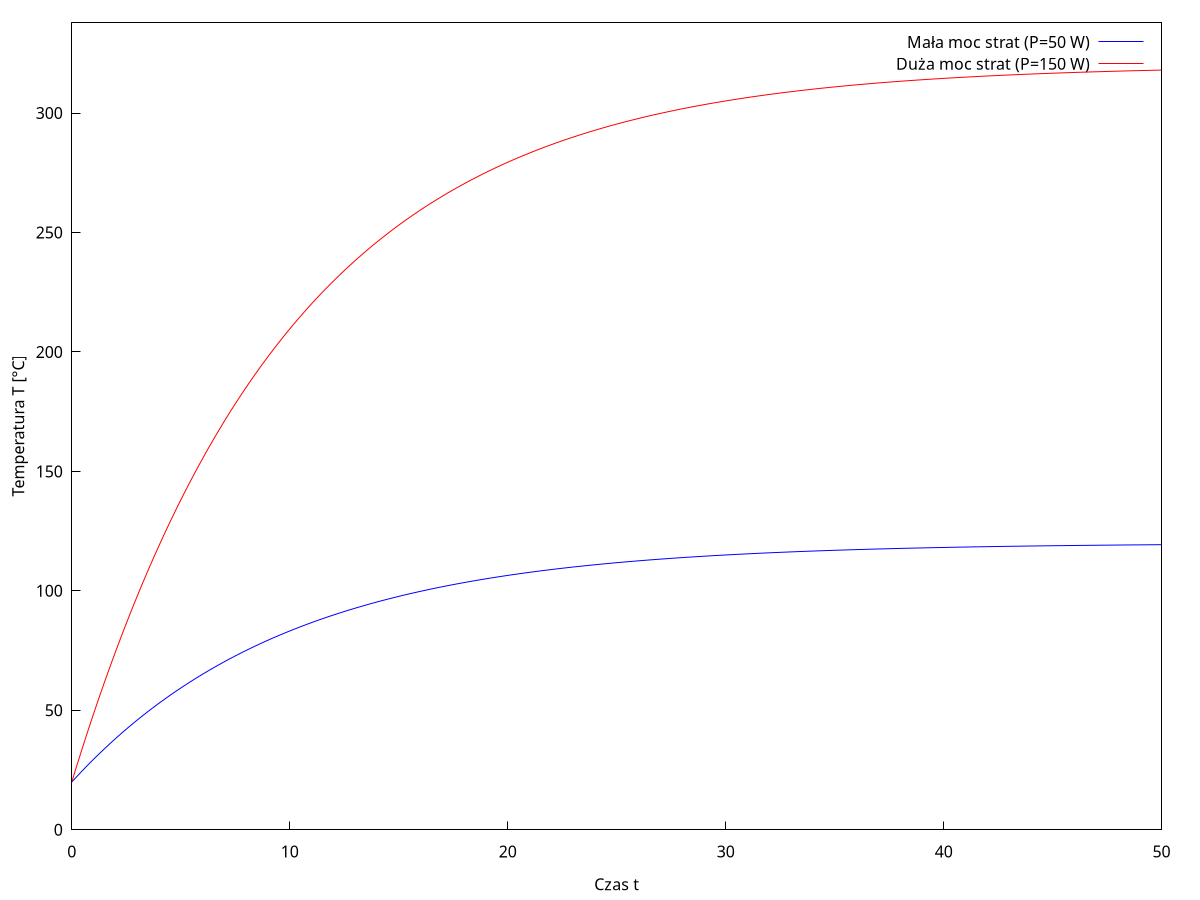
\includegraphics[width=\textwidth]{WYKRES1.png}
		\end{column}
	\end{columns}
	
\end{frame}



\begin{frame}
	\frametitle{Temperatura ustalona silnika $T_\infty(P)$ — wpływ $R_{th}$}
	
	\begin{columns}[T]
		
		% --- Lewa kolumna ---
		\begin{column}{0.42\textwidth}
			\textbf{Cel wykresu}
			\begin{itemize}
				\item analiza wpływu mocy strat $P$,
				\item ocena warunków chłodzenia silnika.
			\end{itemize}
			
			\vspace{0.2cm}
			\textbf{Model analityczny}
			\[
			T_\infty = T_a + P R_{th}
			\]
			
			\vspace{0.15cm}
			\textbf{Parametry}
			\begin{itemize}
				\item $T_a = 20^\circ$C
				\item $R_{th} = 0.5\ \text{K/W}$
			\end{itemize}
			
			\vspace{0.15cm}
			{\footnotesize
				Mała rezystancja termiczna oznacza skuteczne odprowadzanie ciepła,
				dlatego wzrost temperatury wraz z mocą strat jest niewielki.
			}
		\end{column}
		
		% --- Prawa kolumna ---
		\begin{column}{0.58\textwidth}
			\centering
			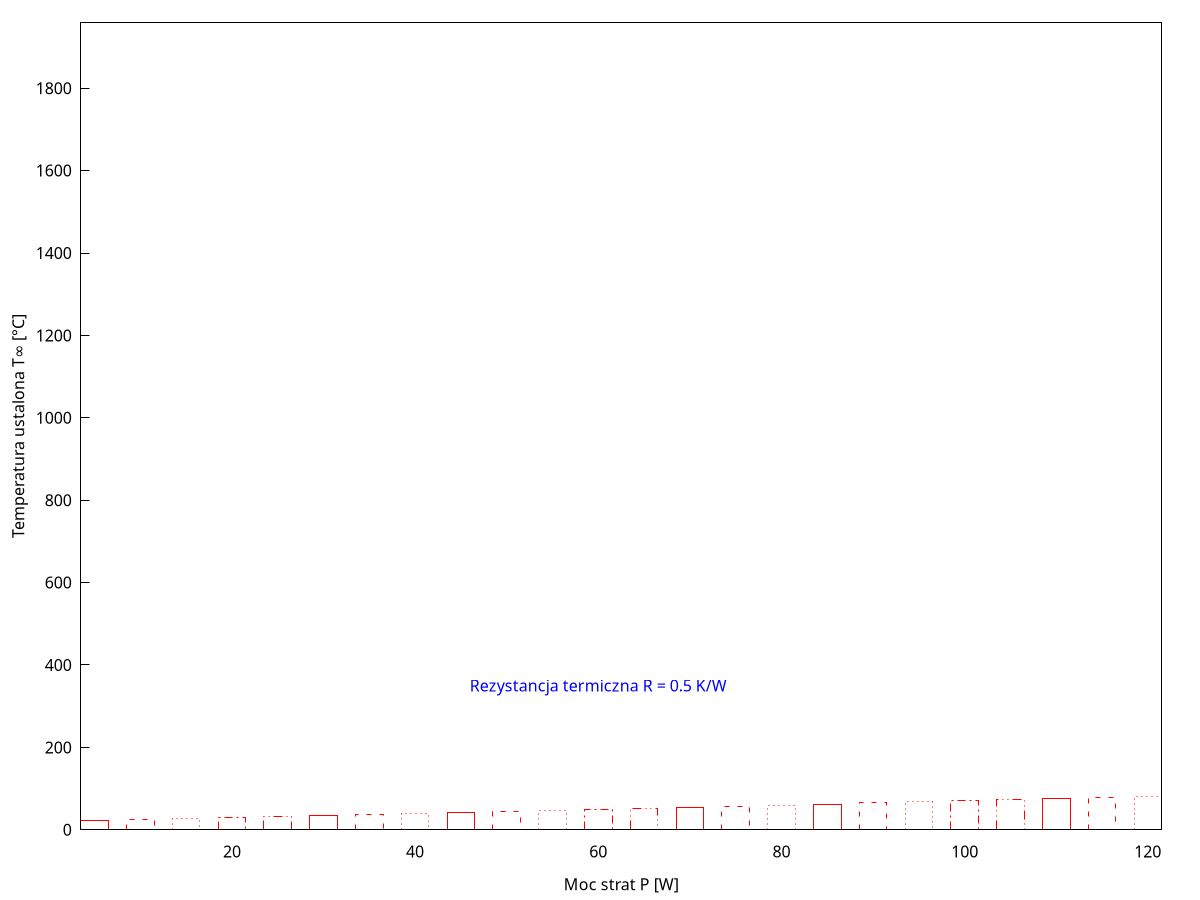
\includegraphics[width=\textwidth]{WYKRES2_1.png}
		\end{column}
		
	\end{columns}
\end{frame}

\begin{frame}
	\frametitle{Temperatura ustalona silnika $T_\infty(P)$ — wpływ $R_{th}$}
	
	\begin{columns}[T]
		
		% --- Lewa kolumna ---
		\begin{column}{0.42\textwidth}
			\textbf{Cel wykresu}
			\begin{itemize}
				\item analiza wpływu mocy strat $P$,
				\item ocena warunków chłodzenia silnika.
			\end{itemize}
			
			\vspace{0.2cm}
			\textbf{Model analityczny}
			\[
			T_\infty = T_a + P R_{th}
			\]
			
			\vspace{0.15cm}
			\textbf{Parametry}
			\begin{itemize}
				\item $T_a = 20^\circ$C
				\item $R_{th} = 1\ \text{K/W}$
			\end{itemize}
			
			\vspace{0.15cm}
			{\footnotesize
				wzrost nachylenia → gorsze chłodzenie
			}
		\end{column}
		
		% --- Prawa kolumna ---
		\begin{column}{0.58\textwidth}
			\centering
			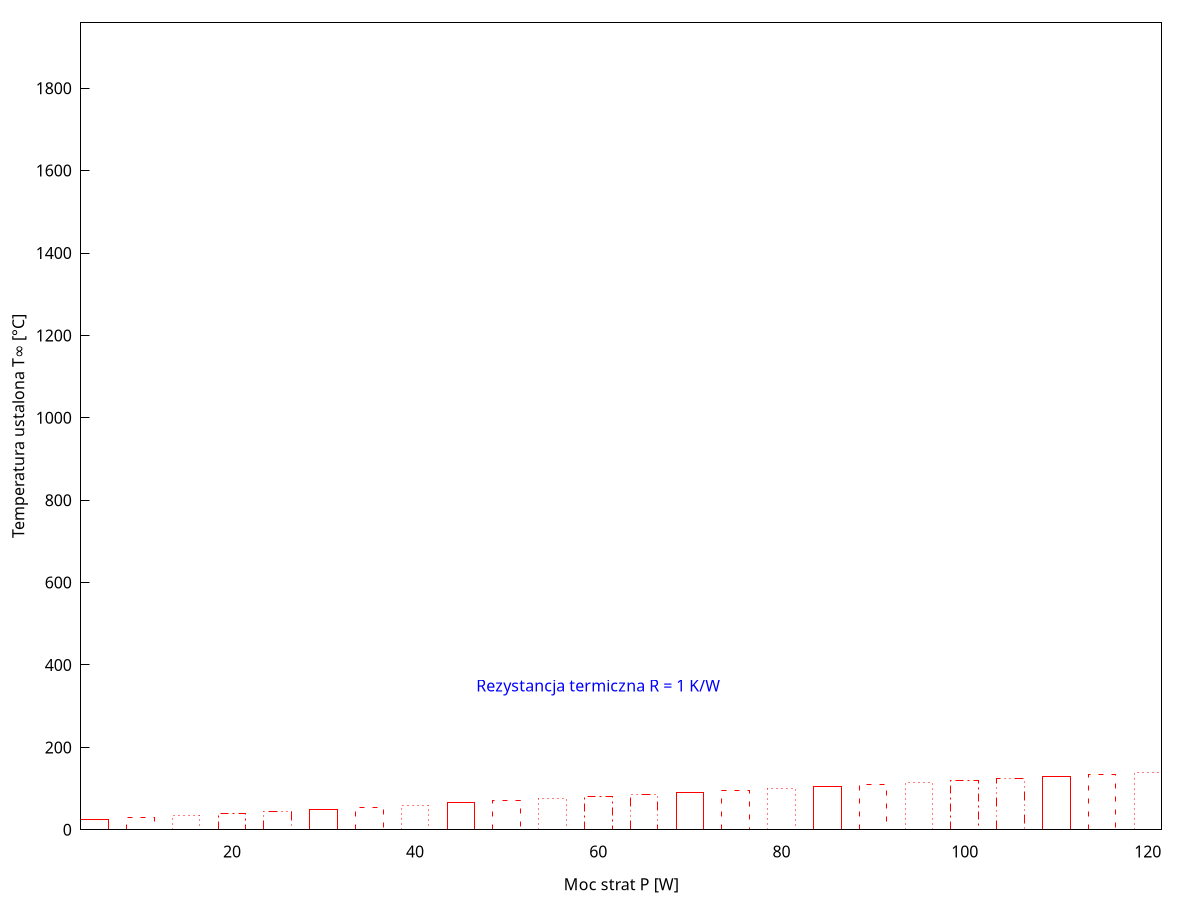
\includegraphics[width=\textwidth]{WYKRES2_2.png}
		\end{column}
		
	\end{columns}
\end{frame}

\begin{frame}
	\frametitle{Temperatura ustalona silnika $T_\infty(P)$ — wpływ $R_{th}$}
	
	\begin{columns}[T]
		
		% --- Lewa kolumna ---
		\begin{column}{0.42\textwidth}
			\textbf{Cel wykresu}
			\begin{itemize}
				\item analiza wpływu mocy strat $P$,
				\item ocena warunków chłodzenia silnika.
			\end{itemize}
			
			\vspace{0.2cm}
			\textbf{Model analityczny}
			\[
			T_\infty = T_a + P R_{th}
			\]
			
			\vspace{0.15cm}
			\textbf{Parametry}
			\begin{itemize}
				\item $T_a = 20^\circ$C
				\item $R_{th} = 2\ \text{K/W}$
			\end{itemize}
			
			\vspace{0.15cm}
			{\footnotesize
				dwukrotnie większa wrażliwość na obciążenie niż dla 1 K/W
			}
		\end{column}
		
		% --- Prawa kolumna ---
		\begin{column}{0.58\textwidth}
			\centering
			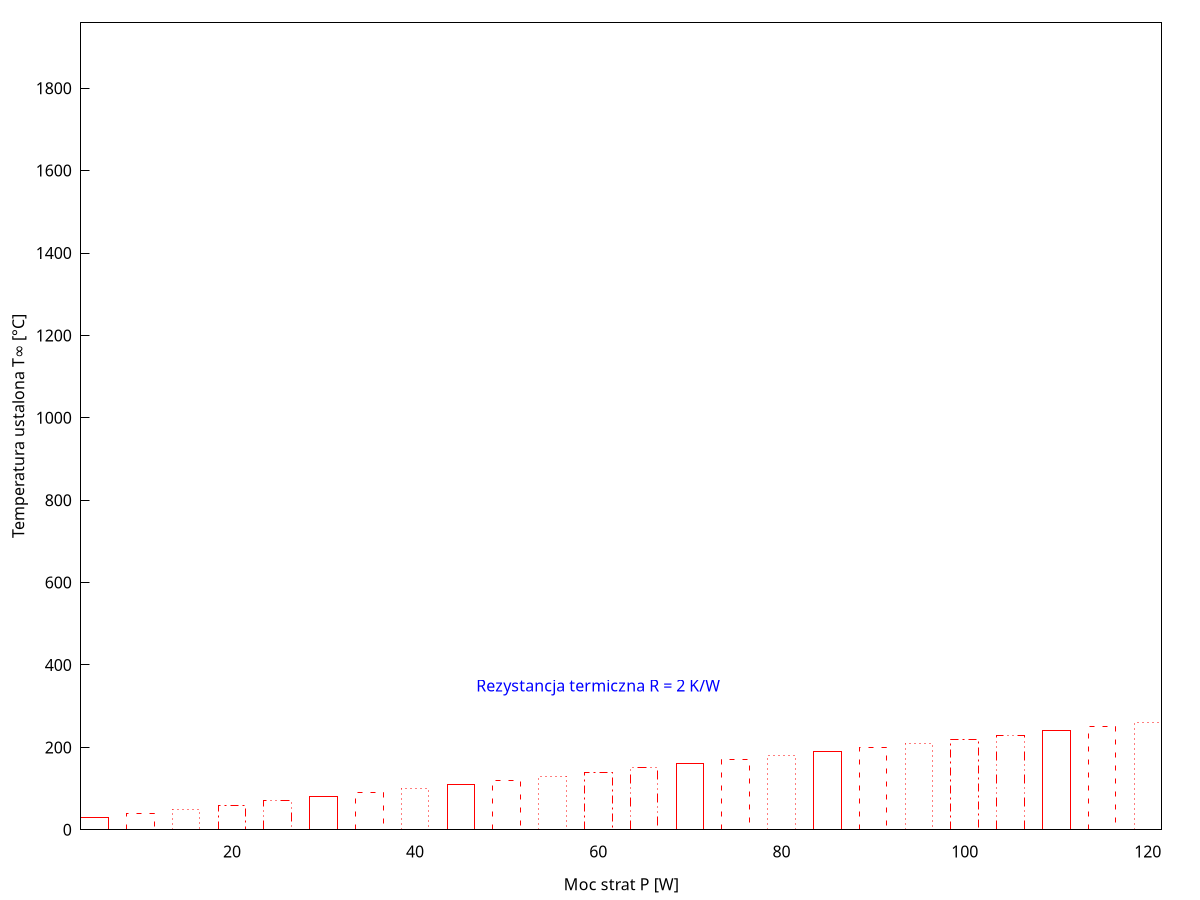
\includegraphics[width=\textwidth]{WYKRES2_3.png}
		\end{column}
		
	\end{columns}
\end{frame}

\begin{frame}
	\frametitle{Temperatura ustalona silnika $T_\infty(P)$ — wpływ $R_{th}$}
	
	\begin{columns}[T]
		
		% --- Lewa kolumna ---
		\begin{column}{0.42\textwidth}
			\textbf{Cel wykresu}
			\begin{itemize}
				\item analiza wpływu mocy strat $P$,
				\item ocena warunków chłodzenia silnika.
			\end{itemize}
			
			\vspace{0.2cm}
			\textbf{Model analityczny}
			\[
			T_\infty = T_a + P R_{th}
			\]
			
			\vspace{0.15cm}
			\textbf{Parametry}
			\begin{itemize}
				\item $T_a = 20^\circ$C
				\item $R_{th} = 4\ \text{K/W}$
			\end{itemize}
			
			\vspace{0.15cm}
			{\footnotesize
				wyraźne ryzyko przegrzewania przy dużym P
			}
		\end{column}
		
		% --- Prawa kolumna ---
		\begin{column}{0.58\textwidth}
			\centering
			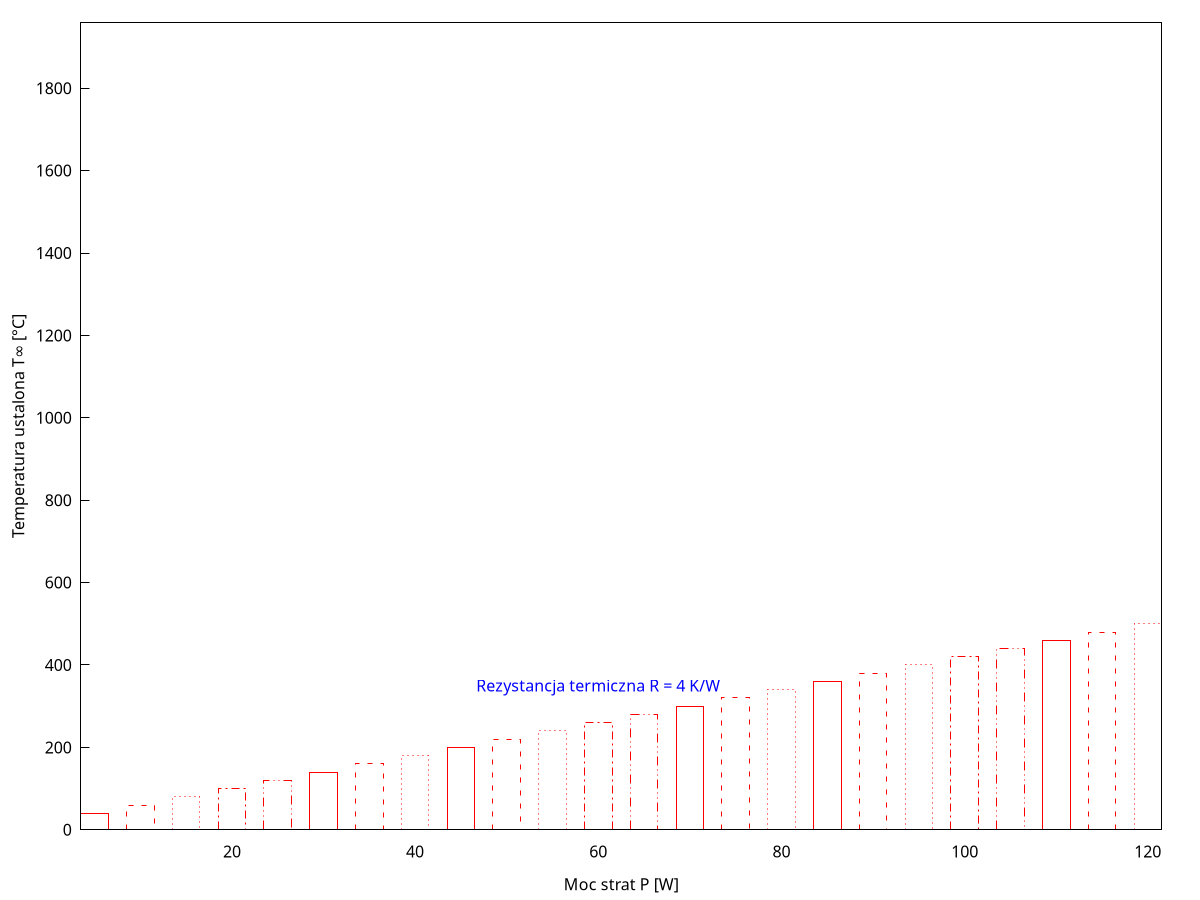
\includegraphics[width=\textwidth]{WYKRES2_4.png}
		\end{column}
		
	\end{columns}
\end{frame}

\begin{frame}
	\frametitle{Temperatura ustalona silnika $T_\infty(P)$ — wpływ $R_{th}$}
	
	\begin{columns}[T]
		
		% --- Lewa kolumna ---
		\begin{column}{0.42\textwidth}
			\textbf{Cel wykresu}
			\begin{itemize}
				\item analiza wpływu mocy strat $P$,
				\item ocena warunków chłodzenia silnika.
			\end{itemize}
			
			\vspace{0.2cm}
			\textbf{Model analityczny}
			\[
			T_\infty = T_a + P R_{th}
			\]
			
			\vspace{0.15cm}
			\textbf{Parametry}
			\begin{itemize}
				\item $T_a = 20^\circ$C
				\item $R_{th} = 8\ \text{K/W}$
			\end{itemize}
			
			\vspace{0.15cm}
			{\footnotesize
				bardzo słabe chłodzenie, stroma charakterystyka
			}
		\end{column}
		
		% --- Prawa kolumna ---
		\begin{column}{0.58\textwidth}
			\centering
			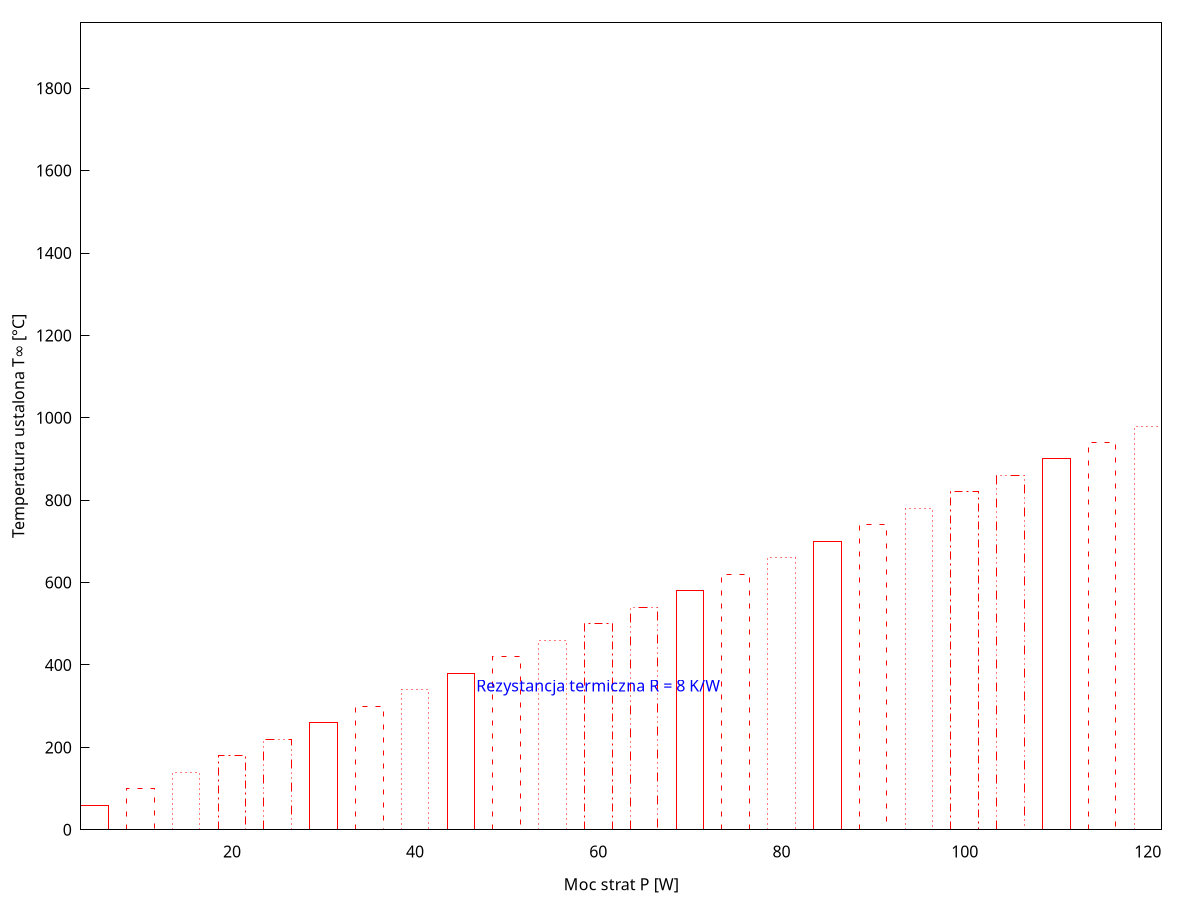
\includegraphics[width=\textwidth]{WYKRES2_5.png}
		\end{column}
		
	\end{columns}
\end{frame}

\begin{frame}
	\frametitle{Temperatura ustalona silnika $T_\infty(P)$ — wpływ $R_{th}$}
	
	\begin{columns}[T]
		
		% --- Lewa kolumna ---
		\begin{column}{0.42\textwidth}
			\textbf{Cel wykresu}
			\begin{itemize}
				\item analiza wpływu mocy strat $P$,
				\item ocena warunków chłodzenia silnika.
			\end{itemize}
			
			\vspace{0.2cm}
			\textbf{Model analityczny}
			\[
			T_\infty = T_a + P R_{th}
			\]
			
			\vspace{0.15cm}
			\textbf{Parametry}
			\begin{itemize}
				\item $T_a = 20^\circ$C
				\item $R_{th} = 16\ \text{K/W}$
			\end{itemize}
			
			\vspace{0.15cm}
			{\footnotesize
				niewielki wzrost mocy powoduje znaczny wzrost temperatury
			}
		\end{column}
		
		% --- Prawa kolumna ---
		\begin{column}{0.58\textwidth}
			\centering
			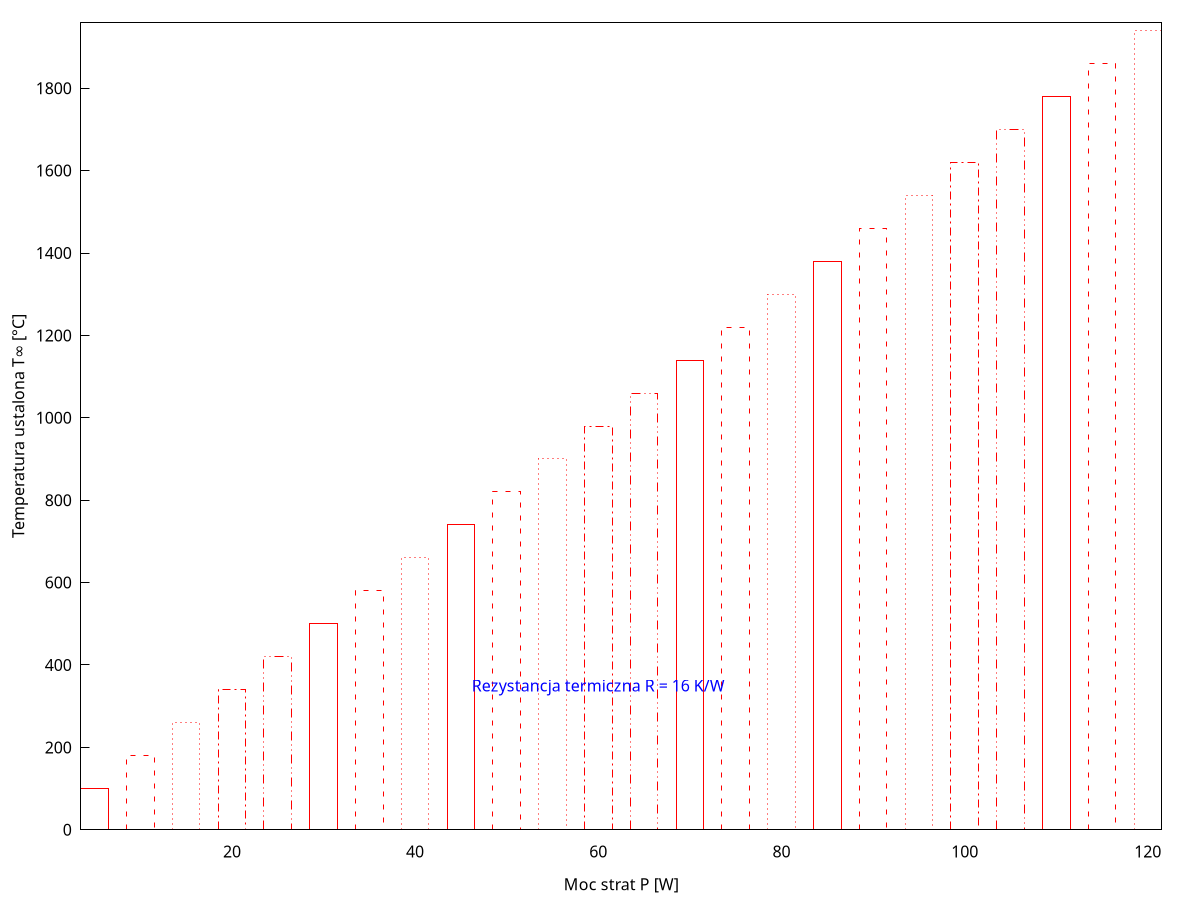
\includegraphics[width=\textwidth]{WYKRES2_6.png}
		\end{column}
		
	\end{columns}
\end{frame}



\begin{frame}
	\frametitle{Wnioski — temperatura ustalona silnika}
	
	\begin{itemize}
		\item Temperatura ustalona $T_\infty$ rośnie liniowo wraz z mocą strat $P$.
		\item Nachylenie charakterystyki zależy wyłącznie od $R_{th}$.
		\item Im większa rezystancja termiczna, tym większa wrażliwość temperatury na obciążenie.
		\item Skuteczne chłodzenie (małe $R_{th}$) znacząco ogranicza ryzyko przegrzania silnika.
	\end{itemize}
	
	\vspace{0.2cm}
	\[
	T_\infty = T_a + P R_{th}
	\]
\end{frame}



\begin{frame}
	\frametitle{Wykres: Wpływ pojemności cieplnej $C_{th}$ na nagrzewanie silnika}
	
	\begin{columns}[T]
		% --- Lewa kolumna: parametry ---
		\begin{column}{0.38\textwidth}
			\textbf{Parametry:}
			\vspace{0.2cm}
			\begin{itemize}
				\item $T_a = 20^\circ$C
				\item $T_0 = 20^\circ$C
				\item $R_{th} = 2\ \text{K/W}$
				\item $P = 100\ \text{W}$
				\item $C_{th} \in \{2,\ 5,\ 10\}\ \text{J/K}$
			\end{itemize}
			
			\vspace{0.25cm}
			{\footnotesize
				Wykres przedstawia przebieg temperatury $T(t)$ w czasie dla różnych
				wartości pojemności cieplnej $C_{th}$.
			}
			
			\vspace{0.15cm}
			{\footnotesize
				Im większa wartość $C_{th}$, tym wolniejsze nagrzewanie silnika,
				przy tej samej temperaturze ustalonej.
			}
		\end{column}
		
		% --- Prawa kolumna: obrazek ---
		\begin{column}{0.62\textwidth}
			\centering
			\includegraphics[width=\textwidth]{WYKRES3.png}
		\end{column}
	\end{columns}
	
\end{frame}
	
	
	
	
	
	
	
	
	
	
	
	
	
\begin{frame}
	\frametitle{Podsumowanie i wnioski}
	
	\begin{enumerate}
		\item \textbf{Model matematyczny:}  
		Zastosowany liniowy model bilansu cieplnego poprawnie opisuje proces nagrzewania silnika elektrycznego.  
		Rozwiązanie równania różniczkowego prowadzi do wykładniczego przebiegu temperatury oraz do istnienia temperatury ustalonej.
		
		\item \textbf{Rola mocy strat $P$:}  
		Moc strat bezpośrednio wpływa na wartość temperatury ustalonej:
		\[
		T_\infty = T_a + P R_{th}
		\]
		\begin{itemize}
			\item Większe $P$ oznacza wyższą temperaturę pracy silnika.
			\item Parametr $P$ jest kluczowy z punktu widzenia bezpieczeństwa eksploatacji.
		\end{itemize}
		
		\item \textbf{Rola pojemności cieplnej $C_{th}$:}  
		Pojemność cieplna wpływa na szybkość nagrzewania silnika:
		\begin{itemize}
			\item Większe $C_{th}$ powoduje wolniejsze zmiany temperatury.
			\item Stała czasowa $\tau = R_{th} C_{th}$ decyduje o dynamice procesu.
			\item $C_{th}$ nie zmienia temperatury ustalonej, a jedynie tempo jej osiągania.
		\end{itemize}
		
		\item \textbf{Znaczenie rezystancji termicznej $R_{th}$:}  
		Rezystancja termiczna wpływa zarówno na:
		\begin{itemize}
			\item poziom temperatury ustalonej,
			\item jak i na szybkość nagrzewania silnika.
		\end{itemize}
		
	\end{enumerate}
	
\end{frame}

	
	
	
	
	
	
	% Slajd: Zakończenie
	\begin{frame}
		\centering
		\vspace{2cm}
		
		{\Huge \textbf{Dziękujemy za uwagę!}}
		
		\vspace{1.5cm}
		

		
		\vfill
		
		\begin{center}
			\small
			Modelowanie nagrzewania silnika elektrycznego z wykorzystaniem równań różniczkowych
		\end{center}
		
	\end{frame}
	
	
	
	
\end{document}